
\documentclass[letterpaper, reqno,11pt]{article}
\usepackage[margin=1.0in]{geometry}
\usepackage{color,latexsym,amsmath,amssymb}
\usepackage{fancyhdr}
\usepackage{amsthm}
\usepackage{mathtools}
\usepackage{tikz}
\usepackage{float}
\usepackage{centernot}
\usepackage{subcaption}
\usepackage{extarrows}
\usetikzlibrary{hobby}
\usetikzlibrary{shapes.multipart}
\usepackage{pgfplots}
\pgfplotsset{compat=1.7}
\usetikzlibrary{arrows.meta}
\usepackage{cancel}
\usetikzlibrary{decorations.markings}
\usetikzlibrary{shapes}
\usetikzlibrary{arrows}
\usepgfplotslibrary{fillbetween}
\usetikzlibrary{patterns}

\newcommand{\RR}{\mathbb{R}}
\newcommand{\CC}{\mathbb{C}}
\newcommand{\ZZ}{\mathbb{Z}}
\newcommand{\QQ}{\mathbb{Q}}
\newcommand{\NN}{\mathbb{N}}
\def\upint{\mathchoice%
  {\mkern13mu\overline{\vphantom{\intop}\mkern7mu}\mkern-20mu}%
  {\mkern7mu\overline{\vphantom{\intop}\mkern7mu}\mkern-14mu}%
  {\mkern7mu\overline{\vphantom{\intop}\mkern7mu}\mkern-14mu}%
  {\mkern7mu\overline{\vphantom{\intop}\mkern7mu}\mkern-14mu}%
  \int}
\def\lowint{\mkern3mu\underline{\vphantom{\intop}\mkern7mu}\mkern-10mu\int}
\DeclareMathOperator{\card}{card}
\DeclareMathOperator{\Binomial}{Binomial}
\DeclareMathOperator{\Span}{span}
\DeclareMathOperator{\sgn}{sgn}
\pagestyle{fancy}
\lhead{Math 321 Lecture 27}
\rhead{Yuchong Pan}
\begin{document}
\pagenumbering{arabic}
\title{Math 321 Lecture 27}
\author{Yuchong Pan}
\date{March 13, 2019}
\newtheorem{thm}{Theorem}
\newtheorem{defn}{Definition}
\newtheorem*{remark}{Remark}
\newtheorem{claim}{Claim}
\newtheorem{cor}{Corollary}
\newtheorem{lemma}{Lemma}
\newtheorem{prop}{Proposition}
\newtheorem{fact}{Fact}
\maketitle
%

\section{HW 9, 3 (b)}

{\bf HW 9, 3 (b):} Find $f \in \mathcal C^{2\pi}$ such that $\sup_N |s_N f(0)| = \infty$.

\medskip

\noindent Assume 3 (a): Given any $n \geq 1$, there exists $f_n \in \mathcal C^{2\pi}$ such that $\lVert f_n \rVert_\infty = 1$ and $\sup_j |s_j f_n(0)| > n$.

\medskip

\noindent {\bf Step 0:} Without loss of generality, we can choose $f_n$ to be a trignometric polynomial, say of degree $d_n$.

\begin{proof}
  Fix $n \geq 1$. Given any $f_n \in \mathcal C^{2\pi}$, we know $\sigma_N(f_n) = \text{$N^\text{th}$ Ces\`aro sum of $f_n$} \xrightarrow[\text{uniformly}]{N \to \infty} f_n$. Fix $N = N_n$ such that
  \[ \lVert \underbrace{\sigma_{N_n} f_n}_\text{a trignometric polynomial} - f_n \rVert_\infty < 1. \]

  \medskip

  \noindent {\bf Note:} $g_n = \sigma_{N_n} f_n$ is a trignometric polynomial.

  \medskip

  We have
  \[ |g_n(x)| \leq \underbrace{|g_n(x) - f_n(x)|}_{\leq 1} + \underbrace{|f_n(x)|}_{\leq 1} \leq 2, \]
  or
  \begin{align*}
    g_n(x) &= \sigma_{N_n} * f_n(x) = \frac{1}{2\pi} \int_{-\pi}^\pi f_n(x - y) K_n(y) dy, \\
    |g_n(x)| &\leq \frac{1}{2\pi} \int_{-\pi}^\pi \underbrace{|f_n(x - y)|}_{\leq 1} \cdot |K_n(y)| dy \leq 1 && \text{because $\lVert K_n \rVert_1 = 1$.}
  \end{align*}
  Suppose $\underbrace{j}_{= e^{cn}}$ is an index such that $\lVert s_{\underbrace{j}_{= e^{cn}}} f_n(0) \rVert > n$. Then,
  \[ |s_n g_n(0)| \geq |s_j f_n(0)| - |s_j (f_n - g_n)(0)| > n - 1, \]
  where
  \begin{align*}
    s_j (f_n - g_n) (\underbrace{0}_{= x}) &= \sum_{k = -j}^j \left[\widehat f_n(k) - \widehat g_n(k)\right] \underbrace{e^{ik\overbrace{x}^{= 0}}}_{= 1}, \\
    |s_j (f_n - g_n) (0)| &\leq \sum_{k = -j}^j \left|\widehat f_n(k) - \widehat g_n(k)\right| \leq 2e^{cn} \cdot \frac{1}{2} e^{cn} = 1, \\
    \left|\widehat f_n(k) - \widehat g_n(k)\right| &\leq \frac{1}{2\pi} \int_{-\pi}^\pi \left|(f_n(x) - g_n(x)) e^{-ikx}\right| dx < 1.
  \end{align*}
\end{proof}

\noindent {\bf Step 1:} We now have a sequence of trignometric polynomials $\{ g_n : n \geq 1 \}$, $\deg(g_n) = d_n$, $\lVert g_n \rVert_\infty \leq 1$, and
\[ |s_{k_n} g_n(0)| > n - 1, \qquad k_n = e^{cn} \ll d_n. \]

\medskip

\noindent {\bf Goal:} Define $f(x) = \sum_{n = 1}^\infty \frac{1}{n^2} \boxed{g_{\lambda_n}(\lambda_n x)}$ for a fast-growing sequence of integers $\lambda_n \nearrow \infty$ to be specified.

Choose $\lambda_n \nearrow \infty$ large enough so that $\lambda_2 > d_1 \lambda_1, \lambda_3 > d_2 \lambda_2, \ldots, \lambda_{n + 1} > d_n \lambda_n$, so non-zero frequencies of individual summands are disjoint.

\medskip

\noindent {\bf Show:} $\sup_N |s_N f(0)| = \infty$.

\medskip

Note that
\begin{align*}
  g_n(x) &= \sum_{k = -d_n}^{d_n} \widehat g_n(k) e^{ikx} && \text{because $g_n$ is a trignometric polynomial}, \\
  g_n(\lambda_n x) &= \sum_{k = -d_n}^{d_n} \widehat g_n(k) e^{i\boxed{k \lambda_n} x} && \text{has frequencies $\{ k\lambda_n : k = 0, 1, \ldots, d_n \}$}.
\end{align*}

\begin{figure}[H]
  \centering
  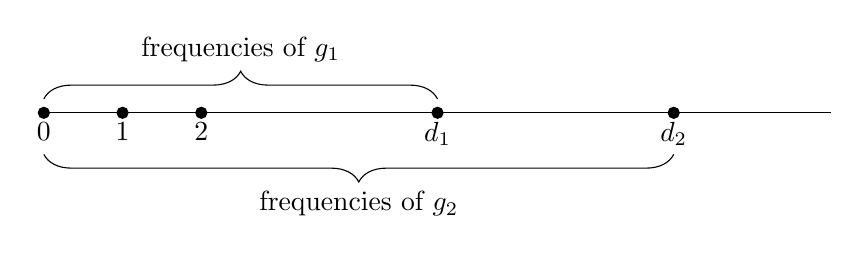
\begin{tikzpicture}
    \draw (0, 0) -- (10, 0);
    \draw[fill=black] (0, 0) circle (2pt) node[below] {$0$};
    \draw[fill=black] (1, 0) circle (2pt) node[below] {$1$};
    \draw[fill=black] (2, 0) circle (2pt) node[below] {$2$};
    \draw[fill=black] (5, 0) circle (2pt) node[below] {$d_1$};
    \draw[fill=black] (8, 0) circle (2pt) node[below] {$d_2$};
    \draw [decorate,decoration={brace,amplitude=10pt}, yshift=5pt] (0, 0) -- (5, 0) node[midway, above, yshift=10pt] {frequencies of $g_1$};
    \draw [decorate,decoration={brace,amplitude=10pt}, yshift=-15pt] (8, 0) -- (0, 0) node[midway, below, yshift=-10pt] {frequencies of $g_2$};
  \end{tikzpicture}

  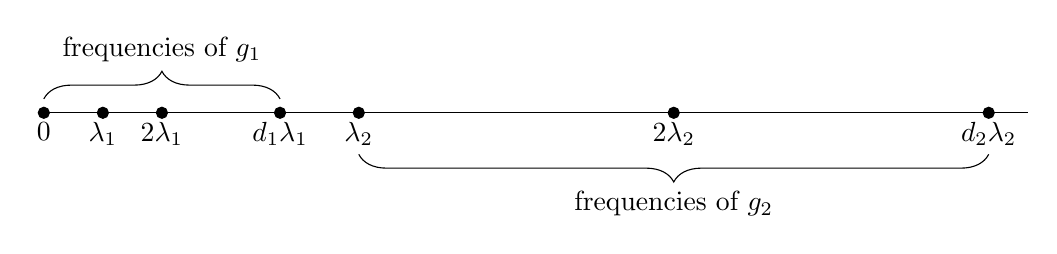
\begin{tikzpicture}
    \draw (0, 0) -- (12.5, 0);
    \draw[fill=black] (0, 0) circle (2pt) node[below] {$0$};
    \draw[fill=black] (0.75, 0) circle (2pt) node[below] {$\lambda_1$};
    \draw[fill=black] (1.5, 0) circle (2pt) node[below] {$2\lambda_1$};
    \draw[fill=black] (3, 0) circle (2pt) node[below] {$d_1 \lambda_1$};
    \draw[fill=black] (4, 0) circle (2pt) node[below] {$\lambda_2$};
    \draw[fill=black] (8, 0) circle (2pt) node[below] {$2\lambda_2$};
    \draw[fill=black] (12, 0) circle (2pt) node[below] {$d_2\lambda_2$};
    \draw [decorate,decoration={brace,amplitude=10pt}, yshift=5pt] (0, 0) -- (3, 0) node[midway, above, yshift=10pt] {frequencies of $g_1$};
    \draw [decorate,decoration={brace,amplitude=10pt}, yshift=-15pt] (12, 0) -- (4, 0) node[midway, below, yshift=-10pt] {frequencies of $g_2$};
  \end{tikzpicture}
\end{figure}

\noindent\fbox{\begin{minipage}{\linewidth}
    \vspace{-.5cm}
    \begin{align*}
      & h_1 + h_2 + \ldots + h_n, \\
      \text{Frequency $k$:} \quad & \widehat h_1(k) + \widehat h_2(k) + \ldots + \widehat h_n(k).
    \end{align*}
\end{minipage}}

\medskip

Choose $\lambda_N \gg N^3$. Then,
\begin{align*}
  s_{\lambda_N^2} f(x) &= \underbrace{s_{\lambda_N^2} \sum_{n = 1}^\infty \frac{1}{n^2} g_{\lambda_n} (\lambda_n x)}_{= a + b}, \\
  |s_{\lambda_N^2} f(0)| &\geq \underbrace{\frac{1}{N^2} s_{\lambda_N^2} g_{\lambda_N} (\lambda_n \cdot 0)}_\text{main} - \underbrace{\left|\sum_{n < N} \frac{1}{n^2} s_{\lambda_n^2} g_{\lambda_n}(0) + \sum_{n > N} \frac{1}{n^2} s_{\lambda_n^2} g_{\lambda_n}(0)\right|}_\text{error} && \text{because $|a + b| \geq |a| - |b|$} \\
  &\geq \frac{1}{N^2} s_{\lambda_N} g_{\lambda_N} (0) \geq \frac{\lambda_N}{N^2} \nearrow \infty.
\end{align*}
Note that
\[ s_{\lambda_N^2} g_N(\lambda_N x) = s_{\lambda_N} g_{\lambda_N} (x). \]

\end{document}
